%\documentclass[12pt,a4paper]{report}
\documentclass[12pt,a4paper,oneside,onecolumn,openright]{book}
% set the document language
\usepackage[italian]{babel}
% set the encoding used by your editor here (default is utf8)
\usepackage[utf8]{inputenc}
\usepackage[T1]{fontenc}

% math packages
\usepackage{amsmath}
\usepackage{amssymb}
\usepackage{multicol}
\usepackage{lmodern}
\usepackage{makecell}
\usepackage[table]{xcolor}
\usepackage{colortbl}

% page margins settings
\usepackage[inner=3cm,outer=2.5cm,top=3cm,bottom=2.5cm]{geometry}
%\usepackage{indentfirst}

% other packages
\usepackage{array}
\usepackage{enumitem}
\usepackage{subfigure}
\usepackage{graphicx}
\usepackage{verbatim}
\usepackage{listings}
\usepackage{url}
\usepackage[hidelinks]{hyperref}
\usepackage[export]{adjustbox}
\usepackage{latexsym}
\usepackage{tabularx}
\usepackage{ragged2e}
\usepackage{mathtools}
\DeclarePairedDelimiter\floor{\lfloor}{\rfloor}
\DeclarePairedDelimiter\ceil{\lceil}{\rceil}
% \usepackage{Mathematics}
% custom colors
\usepackage{color}
\usepackage{wrapfig}
\usepackage{gensymb}
\usepackage{caption}
\usepackage{tikz}
\usepackage{forest}
\usepackage{tikz-qtree}
\usetikzlibrary{positioning, shapes.geometric}
\usetikzlibrary{shapes.geometric, arrows.meta, positioning, fit}
\tikzstyle{block} = [thick, text width=.4cm, minimum height=.5cm, align=center] 


\usetikzlibrary{shadows}
\definecolor{light-gray}{gray}{0.96}
\definecolor{cyan}{RGB}{230,230,255}
\definecolor{dkgreen}{rgb}{0,0.6,0}
\definecolor{gray}{rgb}{0.5,0.5,0.5}
\definecolor{mauve}{rgb}{0.58,0,0.82}
\definecolor{iceberg}{rgb}{0.44, 0.65, 0.82}
% \definecolor{blue}{RGB}{44, 44, 210}

\hypersetup{
colorlinks=true,
linkcolor=black,
% filecolor=blue,
urlcolor=blue,
% pdftitle={Overleaf Example},
}

\urlstyle{same}
\graphicspath{ {./images/} }

\usepackage[many]{tcolorbox}
\newtcolorbox{boxA}{
    % fontupper = \bf,
    boxrule = 1.5pt,
    colframe = black % frame color
}

% environment for bash code
\lstset{ %
  language=bash,                % the language of the code
  basicstyle=\footnotesize,           % the size of the fonts that are used for the code
  numbers=left,                   % where to put the line-numbers
  numberstyle=\footnotesize,          % the size of the fonts that are used for the line-numbers
  stepnumber=1,                   % the step between two line-numbers. If it's 1, each line 
                                  % will be numbered
  numbersep=5pt,                  % how far the line-numbers are from the code
  backgroundcolor=\color{white},      % choose the background color. You must add \usepackage{color}
  showspaces=false,               % show spaces adding particular underscores
  showstringspaces=false,         % underline spaces within strings
  showtabs=false,                 % show tabs within strings adding particular underscores
%  frame=single,                   % adds a frame around the code
  rulecolor=\color{black},        % if not set, the frame-color may be changed on line-breaks within not-black text (e.g. commens (green here))
  tabsize=2,                      % sets default tabsize to 2 spaces
  captionpos=b,                   % sets the caption-position to bottom
  breaklines=true,                % sets automatic line breaking
  breakatwhitespace=false,        % sets if automatic breaks should only happen at whitespace
  title=\lstname,                   % show the filename of files included with \lstinputlisting;
                                  % also try caption instead of title
  numberstyle=\tiny\color{gray},        % line number style
  keywordstyle=\textbf,          % keyword style
  commentstyle=\color{dkgreen},       % comment style
%  stringstyle=\color{mauve},         % string literal style
  escapeinside={\%*}{*)},            % if you want to add a comment within your code
  morekeywords={*,...,insert,-}               % if you want to add more keywords to the setù
}

% environment for python code
\lstset{
	language=Python,
	breaklines=true,
	breakatwhitespace=true ,
	backgroundcolor=\color{light-gray}
}


\newcommand{\grayScale}{0.95} % Can change the gray level here
\definecolor{codeBackground}{rgb}{\grayScale ,\grayScale ,\grayScale}
\definecolor{forestGreen}{rgb}{0.13,0.55,0.13}

\lstset{
    language=C,
    backgroundcolor=\color{codeBackground},
    tabsize=4,
    showstringspaces=false,
    showtabs=false,
    showspaces=false,
    basicstyle=\ttfamily,
    identifierstyle=\ttfamily,
    keywordstyle=\color{blue},
    stringstyle=\color{red},
    commentstyle=\color{gray},
    numberstyle=\color{magenta},
    morecomment=[l][\color{forestGreen}]{\#},
    escapechar={|}, 
}
% appendices package
%\usepackage{appendix}
% set Appendix name used in the toc
%\renewcommand{\appendixtocname}{Appendice}

% interline
\linespread{1.5}
% set numbers for subsections and show them in the toc
\setcounter{tocdepth}{3} 
\setcounter{secnumdepth}{3}

% layout package, style and settings
\usepackage{fancyhdr}
\pagestyle{fancy}

\fancypagestyle{mainmatter}{%		
		\fancyhf{} 
		\fancyhead{}
		\fancyhead[LE,RO]{\thepage}
		\fancyhead[LO]{\footnotesize{\leftmark}}
		\fancyhead[RE]{\footnotesize{\rightmark}}
		\fancyfoot{}
		\addtolength{\headwidth}{\marginparsep}
		\addtolength{\headheight}{2.5pt}
		\renewcommand{\headrulewidth}{0.3pt}
		\renewcommand{\footrulewidth}{0.0pt}
		}
\fancypagestyle{frontmatter}{%
		\fancyhf{} 
		\fancyhead[LE]{\footnotesize{\MakeUppercase{\thepage}}}
		\fancyhead[RO]{\footnotesize{\MakeUppercase{\thepage}}}
		\fancyhead[RE,LO]{}
		\fancyfoot{}
		\addtolength{\headwidth}{\marginparsep}
		\addtolength{\headheight}{2.5pt}
		\renewcommand{\headrulewidth}{0.0pt}
		\renewcommand{\footrulewidth}{0.0pt}
		}
		
		
\usepackage{fancyhdr}
\pagestyle{fancy}
		\fancyhf{} 
		\fancyhead{}
		\fancyhead[LE,RO]{\thepage} 
		\fancyhead[LO]{\footnotesize{\leftmark}}
		\fancyhead[RE]{\footnotesize{\rightmark}}
		\fancyfoot{}
		\addtolength{\headwidth}{\marginparsep}
		\addtolength{\headheight}{2.5pt}
		\renewcommand{\headrulewidth}{0.3pt}
		\renewcommand{\footrulewidth}{0.0pt}

% empty pages have no numbers
\makeatletter
\def\cleardoublepage{\clearpage\if@twoside \ifodd\c@page\else
\hbox{}
  %Potresti voler togliere il commento dalla linea seguente
  %Questa pagina � stata lasciata intenzionalmente vuota.
\thispagestyle{empty}
\newpage
\if@twocolumn\hbox{}\newpage\fi\fi\fi}
\makeatother
%????
%\textwidth=450pt\oddsidemargin=0pt

%\makeatletter 
%  \DeclareRobustCommand*\textsubscript[1]{% 
%    \@textsubscript{\selectfont#1}} 
%  \newcommand{\@textsubscript}[1]{% 
%    {\m@th\ensuremath{_{\mbox{\fontsize\sf@size\z@#1}}}}} 
\makeatother 

\begin{document}
\begin{titlepage}
\begin{center}
{
    \large
    \textbf{Università  degli studi di Modena e Reggio Emilia} \\
   	\textbf{Dipartimento di Ingegneria Enzo Ferrari} \\
    \vspace{\stretch{0.5}}
    \hspace*{0cm} \hrulefill \hspace*{0cm} \\
    \vspace{\stretch{0.5}}    
	  \vspace{\stretch{12}}
  
  
 		\huge{\bf Automotive Connectivity }}\\
		\vspace{3mm}
		
		\vspace{\stretch{6}}
		\end{center}
		
\vspace{40mm}
\par
\noindent
\vspace{20mm}
\begin{center}
\hspace*{0cm} \hrulefill \hspace*{0cm} \\
{\large{\bf 
Anno Accademico 2024/25}}
\end{center}

\end{titlepage}

\pagestyle{frontmatter}
\frontmatter

% PAGINA VUOTA
%\clearpage\null\thispagestyle{empty}\clearpage
\setcounter{tocdepth}{2}
\tableofcontents

\setlength{\parindent}{12pt}
\setlength{\parskip}{1ex plus 0.5ex minus 0.2ex}
\mainmatter
\pagestyle{mainmatter}

\chapter{Introduction}

\section{Structure and Content}
\begin{itemize}

    \item \textbf{Module 1}: 
    \begin{enumerate}
        \item \textbf{\textit{intra-vehicles communications}}: nodes, sensors, ECU
        \item \textbf{\textit{signal busses}}: CAN, LIN, FlexRay, MOST, Ethernet [ T1/T1S]
        \item \textbf{\textit{car domain and OS}}
    \end{enumerate}
    
    \item \textbf{Module 2}:
    \begin{enumerate}
        \item \textbf{\textit{inter-vehicles communications}}: \textit{V2V} and \textit{V2X} (car is a node)
        \item \textbf{\textit{wireless technologies}}: Bluetooth, LoRa, C-V2X, IEE 802.11p (bd)
        \item application, messages, broadcast, GPS
    \end{enumerate}

\end{itemize}
Different \textbf{domain} or \textbf{application} needs different \textit{communications protocols}, is important to understand how each nodes in domain communicate each other (inside the car).

\newpage
\section{Intra-Vehicles}
From the 80's, where the car's control unit are isolated an there was a dedicated wires connect sensors and actuators with less electronic than now, until the reach the greates goal of evolution in the automotive sector: autonomous drive. The complexity of the number of connection from each ECU's to the other, also the number of ECU's for each car, is growing. While the number of signal increase in a liner way, the connection between ECU's is growing with a quadratic complexity $O(n^2)$.

If we examine the evolutions of the ECUs number inside an ``Audi A6'' we can observe that in 1997 it has 5 ECUs and in the 2007 it has 50 ECUs, instead the ``Tesla M3'' in the 2017 has 70 ECUs. The quadratic increase of ECUs number, however has reach a cap for two main reason: the cost and the space inside the car. Traditionally one ECUs is responsible of one task, but nowadays it could be two type of trends:
\begin{enumerate}[nosep]
    \item \textit{distributed of function across ECUs}
    \item \textit{integration of multiple function in one ECU}
\end{enumerate}

\section{Architectures}

\begin{figure}[h]
    \centering
    \begin{minipage}[t]{0.45\textwidth}
        \centering
        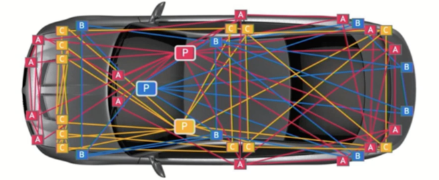
\includegraphics[width=\textwidth]{img/domain_architecture}
        \caption{\textit{Domain Architecture}}
        
        \begin{flushleft}
            \begin{enumerate}[nosep]
                \item central domain controller (\textbf{P}) or high performance computer
                \item ability to handle more complex functions
                \item cost optimization
                \item cable harness is rigid and expensive
            \end{enumerate}
        \end{flushleft}

    \end{minipage}
    \begin{minipage}[t]{0.45\textwidth}
        \centering
        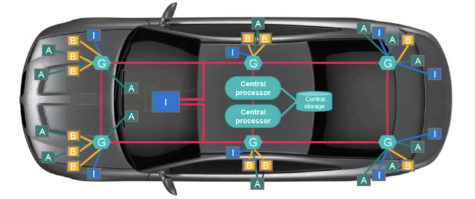
\includegraphics[width=\textwidth]{img/zonal_architecture}
        \caption{\textit{Zonal Architecture}}
        
        \begin{flushleft}
            \begin{enumerate}[nosep]
                \item local ethernet per zone (\textbf{G})
                \item ultra high-speed secured backbone between zone
                \item centralized software
                \item central computer storage
            \end{enumerate}
        \end{flushleft}
        
    \end{minipage}
\end{figure}
\chapter{Intra-Vehicles}

\section{ISO/OSI Layers}
In telecommunication the idea is to divide each steps into layers starting from the application layer to the fisical ones, every layers have different function and it needs different protocols. Each layer can interact with the one that is above or below it and the communication of two layers follow rigid and specifics rules. Nowadays the standard \textit{de iure} is the \textbf{ISO/OSI}, instead the the \textit{de facto} standard is the \textbf{TCP/IP} that relax the rigid guidelines. The \textit{ISO/OSI} has seven layers (bottom to top):
\begin{enumerate}[nosep]
    \item \textbf{physical layer}: specifies the mechanical and electrical properties to transmit bit (in the ``real'' world) and to control time synchronization.
    \item \textbf{data link layer}: checked the transmission of the frame, error checking, frame synchronization and flow control.
    \item \textbf{network layer}: it is used for the transmission of the packets, it is also know as \textit{IP Layer}, in is normally use in ethernet.
    \item \textbf{transport layer}: reliable end to end transport segment, you can manage how the data have to flow. In 99.99 \% of the car domain it doesn't need.
    \item \textbf{session layer}: establish and tear down sessions.
    \item \textbf{presentation layer}: define the syntax and the semantics of information.
    \item \textbf{application layer}: uses data transmitted via physical medium.
\end{enumerate}
In the first module we need only two layers: \textbf{physical layer} and \textbf{data link layer}. We have to study the behaviour of the communication protocols like CANBus, LIN, FlexRay, MOST and Ethernet in this two layers. Starting from the \textbf{transmission medium}, normally the hardware pieces that we use to interact with is:
\begin{itemize}[nosep]
    \item \textbf{transceiver}: is used to ``convert'' analog signal to bits (brain less).
    \item \textbf{controller}: control the communication (brain full).
\end{itemize}
Initially the idea is to focus a little more on \textbf{CANBus}, the \textbf{\textit{Physical Layer}}: is compose by three component: \textbf{Physical Signaling - PLS}, \textbf{Physical Medium Attachment - PMA} and \textbf{Media Dependant Interface - MDI}.
\begin{enumerate}[nosep]
    \item \textbf{physical signaling}: the main purpose is to understand the bit encoding/decoding (if it is \textit{NRZ} or \textit{Manchester}) and to mantein the synchronization all over the network, every transceiver it must have a the same clock source. The synchronization is the most important things both for the bit encoding/decoding and for don't introduce delay in the communication.
    \item \textbf{physical medium attachment}: driver/receiver characteristics based on the communication protocol.
    \item \textbf{media dependant interface}: the connector for access to the physical medium.
\end{enumerate}
\textbf{\textit{Data Link Layer}} is compose by two component: \textbf{Logical Link Control - LLC} and \textbf{Medium Access Control - MAC}.
\begin{enumerate}[nosep]
    \item \textbf{logical link control}: from now on, we start to call \textit{frame} the data that are send/receiver from the physical channel. It is used for \textit{acceptance filtering} that permit to decide if a frame is important for the application above the \textit{controller} and if not discard it. This component include also the \textit{overload notification} and \textit{recovery management} in the case there is an error on the communication they could ask to a re-transmit the data.
    \item \textbf{medium access control}: is purpose is \textbf{error detection} it could check the data encapsulation/decapsulation, frame coding and error detection/signaling/handling.
\end{enumerate}

\section{Network Topology - The Bus System}
\begin{figure}[h]
    \centering
    \begin{minipage}[t]{0.3\textwidth}
        \centering
        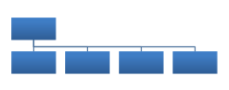
\includegraphics[width=\textwidth]{img/line}
        \caption{\textit{Line Topology}}
        
        \begin{flushleft}
            In the \textbf{Line} topology also know like \textbf{\textit{Bus}} topology each node is connected by interface connectors to a single center cable. It is cheaper than the others and it has lower complexity but it is not very robust.
        \end{flushleft}

    \end{minipage}
    \begin{minipage}[t]{0.3\textwidth}
        \centering
        
\includegraphics[width=\textwidth]{img/star}
        \caption{\textit{Star Topology}}
        
        \begin{flushleft}
            In the \textbf{Star} topology every peripheral nodes is connected to a central node called \textit{hub} or \textit{switch}. It has an higher cost and complexity than the \textit{bus} topology, but it is much more robust (if the \textit{hub} goes down it is a \textit{single point of failure}).
        \end{flushleft}
        
    \end{minipage}
    \begin{minipage}[t]{0.3\textwidth}
        \centering
        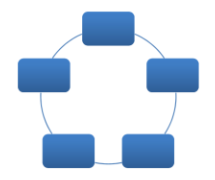
\includegraphics[width=\textwidth]{img/ring}
        \caption{\textit{Ring Topology}}
        
        \begin{flushleft}
            The \textbf{Ring} topology is a \textit{daisy chain} in a closed loop. When a node sends data to another, the data passes through each intermediate node on the ring until reach its destination (it use only one direction). It is not too munch expensive, but has higher complexity (if you want add a new node it could be troublesome).
        \end{flushleft}
        
    \end{minipage}
\end{figure}
In the autonomotive domain it is chosen the \textbf{\textit{Bus Topology}}, why? The first thing is that in the automotive industry it is mandatory to maintain lower the cost. The \textit{busses} are very cheap for the materials, the weight and the volume. In the \textit{bus} topology it is possible to have higher modularity, you can \textit{plug \& play} a node ``when you want'', in that way it is possible to have fully customizability inside the vehicles. The last things is that there is shorter development cycles.
In the autonomotive field there is three main component:
\begin{enumerate}[nosep]
    \item \textbf{\textit{transceiver}}: it is the \textit{physical layer definition} and implement the first layer of the \textit{ISO/OSI} stack.
    \item \textbf{\textit{communication controller}}: it is the communication protocol and implement the first and the second layers of the \textit{ISO/OSI} stack.
    \item \textbf{\textit{ECU}}: also know like \textbf{electronic controller unit} and implement the last layer of the \textit{ISO/OSI} stack, the \textbf{application} layer.
\end{enumerate}
The idea is to made possible to abstract the application layer in order to, if you want, change the first two layers, for example from CANBus to FlexRay, but nothing change at the application layer.

\section{Controller Area Network}
The \textbf{Controller Area Network} also know as \textbf{CAN} is a vehicle bus standard to enable efficient communication. It is originally developed to reduce complexity and cost of electrical wiring. \textbf{\textit{CANBus}} use an \textbf{electrical} medium over wires and a \textbf{broadcast} data transmission. CANBus use the \textbf{\textit{CSMA/CR}} like \textit{multiple access protocol}, it means \textit{carrier sense multiple access collision resolution} protocol, that permit to CANBus to have \textbf{\textit{arbitration}} on the channel access. In this way there is random access to the physical channel, but it is impossible that there is some collision on the communications.
\begin{figure}[h]
    \centering
    \label{img:canbus_1}
    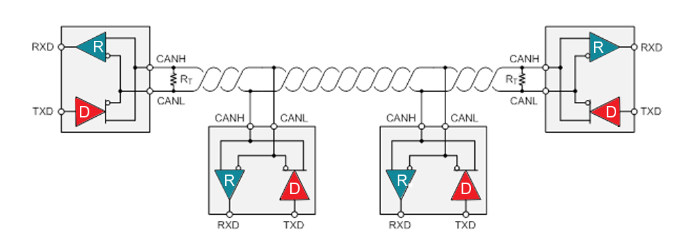
\includegraphics[width=0.75\textwidth]{img/canbus_1}
    \caption{CANBus Network Topology}
\end{figure}

The \textbf{CANBus} network is compose by two wires: \textbf{CAN High} and \textbf{CAN Low}. The data is transmit over the wire using the \textit{potential difference} on each transceiver. Two twisted wires are use because it gives to the protocol \textbf{noise resistance} and \textbf{increase resiliency}, if one brakes, CAN Low \textit{survives}. At the end of the wire in the bus topology there are place two impedance $R_T$ of $120\ohm$. Each CANBus node has three element:
\begin{itemize}[nosep]
    \item \textbf{CAN Transceiver}: is directly connected to the medium access by two pin (one on CANH and the other on CANL). It has the goal to translate the voltage level into bits (during the reception) and send it to the \textit{CAN Controller} and translate bit into voltage level (during the  transmission).
    \item \textbf{CAN Controller}: is connect to the \textit{CAN Transceiver} by two pin (CANTX and CANRX) and is scope is to: message completion, control bus access, transmission and reception of the message, bit timing.
    \item \textbf{Microcontroller}: application software communicating with other ECUs via messages over the bus.
\end{itemize}

\begin{tabular}{ ||p{1cm}|p{2cm}|p{1cm}|p{2cm}|p{2cm}|p{2cm}|p{1cm}|p{1cm}|| } 
    \hline
    \multicolumn{8}{|c|}{ \textbf{CAN Message} } \\ \hline
    1 bit & 29 bit & 1 bit & 6 bit & 0-64 bit & 16 bit & 2 bit & 7 bit\\ \hline
    SOF & CAN-ID & RTR & Control & Data & CRC & ACK & EOF \\ \hline
\end{tabular}

\begin{itemize}[nosep]
    \item \textbf{SOF}: is the \textbf{start of frame} is always set to \textit{dominant \textbf{0}} to tell the other ECUs that a message is coming.
    \item \textbf{CAN-ID}: contains the message identifier - lower value have higher priority.
    \item \textbf{RTR}: is the \textbf{remote transmission request} allow to ECUs to ``request'' message from other ECUs.
    \item \textbf{Control}: informs the lenght of the \textit{Data} in bytes (0 to 8 bytes), two bits are \textit{reserved} for future implementation.
    \item \textbf{Data}: contains the actual data values, which need to be ``scaled'' or converted to be readable an ready for analysis.
    \item \textbf{CRC}: is the \textbf{cyclic rendundancy check} is used to ensure data integrity.
    \item \textbf{ACK}: is the \textbf{acknoledgement} this slot indicates if the CRC is OK all the bits must be \textbf{recessive} (\textit{logical 1}).
    \item \textbf{EOF}: is the \textbf{end of frame} marks the end of CAN message all the bits must be \textbf{recessive} (\textit{logical 1}).
\end{itemize}
The CANBus use a \textit{message passing} technologies, it means, when a message is sent through the wire by an ECUs all the CAN Transceiver reciver the message, but if a application layer of one of another ECUs doesn't need that message it could ignore or if it need it, it could accept that message, using the \textit{CAN-ID} as identifier. In other word the CANBus use the \textbf{receiver-selective} form of addressing. In the CANBus the bit logic is pretty simple, each ECUs reads the wire (through a buffer) and each ECUs \textbf{can} write on the line (through a transistor), in this way the \textbf{basic state} is \textbf{up} ($+5V$ or logical ones) when one or more ECUs want to set signal low turn on transistor conductive (diode), this connect the bus to signal ground in this case the bus level is \textbf{low} ($0V$, or logical zeros) indipendently from other ECUs. The \textbf{0} is named \textbf{dominant level}. It could be see the CANBus wires as \textbf{logical AND} (if an ECUs write zeros the state is \textit{zeros}). \\ \newline
The CANBus is an \textbf{event-driven} bus system, it means that there is no need to wait a scheduled time slot for sending data and there is the possibility of collision over the communication channel. If an ECU $X$ registers an event $e$ it is authorized to access the busses immediately and send data, but if another ECU $Y$ is alredy transmitting data, then $X$ waits. We want to calculate how long it takes a message to be sent, the first thing to do is to calculate the maximum bits number that is allow in a CAN Message: 130 bits. The CANBus can have lots of different bus speed $B \in \{5 k \cdot \frac{bit}{s}, 125 k \cdot \frac{bit}{s}, 250 k \cdot \frac{bit}{s}, 500 k \cdot \frac{bit}{s}, 800 k \cdot \frac{bit}{s}, 1 M \cdot \frac{bit}{s}\}$, let's consider the average $B = 500 k \cdot \frac{bit}{s}$, the resulting time for sending a message is equal to $T_x(time) = \frac{M}{B} = \frac{130 bit}{500 k \cdot \frac{bit}{s}} = 0.25 ms$, but what is happen if two ECUs start the communication on the same time? Let's consider the case where there are three ECUs $X, Y, Z$, $X$ and $Y$ are waiting $Z$ because it is using the medium access, but probably they start to transmit in the same time when the busses is free, in this case we have a \textbf{collision}, the solution is how CANBus implement the \textbf{\textit{CSMA-CR}}, \textbf{carrier sense multiple access - collision resolution}, the two ingredients are how we can see the CAN busses (like a logical AND) and the \textbf{CAN-ID} to the logic prioritizing.
\begin{enumerate}[nosep]
    \item ECU $X$ want to send: it must check if the bus is free (\textit{carrier sense} - \textbf{CR}).
    \item if it is busy the ECU have to wait.
    \item when the bus is free, it could happen that one or more ECUs are ready to transmit, and start the communication together (\textit{multiple access} - \textbf{MA}).
    \item the last incredient is how to avoid the impending damage born from the collsion? (\textit{collision resolution} - \textbf{CR}) $\rightarrow$ \textbf{\textit{bitwise arbitration}}.
\end{enumerate}

All the \textbf{\textit{bitwise arbitration}} is base on the first two field of the CANBus Message: \textbf{SOF} (it is for everyone a \textbf{dominant bit}: \textbf{\textit{0}}) and \textbf{CAN-ID} (it could be 11 bits, in the standard CANBus and 29 bits for the extended ones). We know that in CANBus the ones with the lower \textit{ID} has the greatest priority. Another basic know is that the CANBus network work like a \textit{wired-AND} so if a nodes wrote on the bus a \textbf{\textit{0}} the entire network has logically low value, also if someone else try to wrote a logically high value.

\begin{center}
    \begin{tabular}{ | c | c | c | c | c | c | c | c | c | c | c | c | } \hline
        & \textbf{ID 10} & \textbf{ID 9} & \textbf{ID 8} & \textbf{ID 7} & \textbf{ID 6} & \textbf{ID 5} & \textbf{ID 4} & \textbf{ID 3} & \textbf{ID 2} & \textbf{ID 1} & \textbf{ID 0} \\ \hline
        \textbf{A} & 1 & 1 & 0 & \textcolor{red}{\textbf{0}} & 1 & 0 & 0 & 1 & 1 & 0 & 0 \\ \hline
        \textbf{bus} & 1 & 1 & 0 & \textcolor{red}{\textbf{\textit{0}}} & 1 & 0 & 0 & 1 & 1 & 0 & 0 \\ \hline
        \textbf{B} & 1 & 1 & 0 & \textbf{1} & \multicolumn{7}{ | c }{\makecell{node B loses \textit{arbitration} \\ $\rightarrow$ stop sending and re-start sensing}} \\ 
        \cline{1-5}
    \end{tabular}
\end{center}

\begin{figure}[h]
    \centering
    \begin{minipage}[t]{0.45\textwidth}
        \begin{tabular}{ | c | c | c | } \hline
            \multicolumn{3}{ | c | }{\textbf{wired-and bus logic}} \\ \hline
            \textbf{sender $a$} & \textbf{sender $b$} & \textbf{bus level} \\ \hline
            1 & 1 & 1 \\ \hline
            1 & \textcolor{red}{0} & \textcolor{red}{0} \\ \hline 
            \textcolor{red}{0} & 1 & \textcolor{red}{0} \\ \hline
            \textcolor{red}{0} & \textcolor{red}{0} & \textcolor{red}{0} \\ \hline
        \end{tabular}
        \begin{flushleft}
            We have three knowledge: the default value of the CANBus network is logically high, the bus work as \textit{wired-AND} and the logic \textbf{\textit{0}} si the \textbf{dominant} value, so if the \textit{sender a} or \textit{sender b} send over the bus the \textbf{\textit{0}} value, it win the \textit{arbitration} with the other \textit{sender}.
        \end{flushleft}
    \end{minipage}
    \begin{minipage}[t]{0.45\textwidth}
        \begin{tabular}{ | c | c | c | } \hline
            \multicolumn{3}{ | c | }{\textbf{arbitration logic}} \\ \hline
            \textbf{sender} & \textbf{bus} & \textbf{interpretation} \\ \hline
            0 & 0 & \textbf{next} \\ \hline
            0 & 1 & \textbf{\textit{fault}} \\ \hline
            1 & 0 & \textbf{\textcolor{red}{stop}} \\ \hline 
            1 & 1 & \textbf{next} \\ \hline
        \end{tabular}
        \begin{flushleft}
            We alredy know that CANBus is \textit{carrier sense} if the sender sent over the network a logical \textbf{\textit{1}} but read logical \textbf{\textit{0}} knows that it losts the \textit{arbitration} with another \textit{sender} and have to stops the transmission.
        \end{flushleft}
    \end{minipage}
\end{figure}

\textbf{\textit{Priorities instead of Collision}}: the bus logic and arbitration logic not only prevent collision, it ensure a priority-controlled bus access: smaller ECUs ID, higher priority.
\newpage
\textbf{\textit{CANBus Message Integrity}}: the idea is to use the Data field to generate a CRC to permit the check on the integrity of the message, but wee need some basic knowledge before start: \textit{polynomial division} and \textit{XOR}. 
\begin{boxA}
    \textbf{\textit{Polynomial Reminder Theorem}}: given two polynomials $M(x)$ (the dividend) and $G(x)$ (the divisor), asserts the existence (and the uniqueness) of a quotient $Q(x)$ and a remainder $R(x)$ such that:
    \begin{center}
        \begin{math}
            M(x) = Q(x) \cdot G(x) + R(x)
        \end{math}
    \end{center}
    N.B. the degree of $R(x)$ is stricly lower than the degree of $G(x)$.
\end{boxA}
In the calculation of \textit{CRC} depends on the arithmetic of modulo 2 polynomial. A modulo 2 polynomial is like:
\begin{center}
    $a_n \cdot x^n + a_{n-1} \cdot x^{n-1} + ... + a_2 \cdot x^2 + a_1 \cdot x + a_0$ \\
    $a = \{0, 1\} \quad \forall a \in \{a_0, a_1, ..., a_n\}$
\end{center}
An example of the representation of a binary polynomial is like: $x^3 + x + 1 = 1011$. If exist an $x$ with a certain exponent $e$ like: $x^e$ in the binary representation the position $e$ is fill with a $1$. \\
\begin{center}
    \begin{tabular}{ | c | c | c | } \hline
        $\oplus$ & \textbf{0} & \textbf{1} \\ \hline
        \textbf{0} & 0 & 1 \\ \hline
        \textbf{1} & 1 & 0 \\ \hline
    \end{tabular}
\end{center}
The \textbf{\textit{XOR}} is a digital logic gate that gives a true (logical 1) when the input number is odd, otherwise is false (logical 0). \\ \newline
\textbf{\textit{CRC Encoding}}:
\begin{enumerate}[nosep]
    \item we need to transmit a \textit{n bits} \textbf{message} $M(x)$: $deg(M(x)) = n - 1$.
    \item we have a \textit{m + 1 bits} \textbf{generator} $G(x)$: $deg(G(x)) = m$.
    \begin{itemize}[nosep]
        \item the \textbf{remainder} $R(x)$ of the division $\frac{M(x)}{G(x)}$ will have strictly lower degree respect to $G(x)$ and, in the worst case, the maximum value will be $deg(R(x)) = m - 1$.
        \item $R(x)$ can always expressed with $m$ bits.
    \end{itemize}
    \item add $m$ zeros at the end of $M(x)$: this means to do the following $M(x) \cdot x^m$.
    \item divide the \textbf{new message} $M(x) \cdot x^m$ with the \textbf{generator} $G(x)$ to obtain the \textbf{\textit{reminder}} of \textit{m} bits called \textbf{\textit{CRC}}.
    \item the final message $B(x)$ is equal to $M(x) \cdot x^m + CRC$: this means to add the CRC bits at the end of the message replacing the $m$ zeros padded before.
\end{enumerate}
\textcolor{green}{\textbf{Example}}:
\begin{center}
    $M(x) = 1101011011 \qquad G(x) = 10011 \quad (m = 4)$ \\
    $M(x) \cdot x^m = 11010110110000$
\end{center}
\begin{figure}[h]
    \centering
    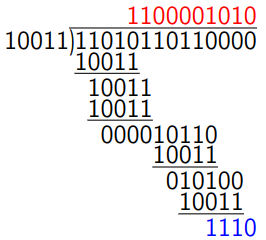
\includegraphics[width=0.3\textwidth]{img/crc_cal}
\end{figure}
The final message $B(x)$ is equal to: $B(x) = \underbrace{1101011011}_\text{M(x)}\underbrace{10011}_\text{R(x)}$ \\ \newline
\textbf{\textit{CRC Decoding}}
\begin{enumerate}[nosep]
    \item the receiver \textbf{acquire} $B(x) = M(x) \cdot x^m + CRC$.
    \item the receiver \textbf{knows} $G(x)$.
    \item the receiver \textbf{divides} the whole message by the generator: $B(x) = \frac{M_x \cdot x^m + CRC}{G(x)}$ 
    \item if the receiver obtain \textbf{no reminder} the transmission was successfully (no errrors detected).
\end{enumerate}
\textbf{\textit{CRC Error Resistance}}: consider an error $E(x)$ occurs on the transmission channel and the receiver $B(x) + E(x)$ instead of simply $B(x)$, when the \textit{CRC logic} can failed? The problem occure when $E(x)$ is multiple of $G(x)$ in this way $\frac{B(x) + E(x)}{G(x)}$ gives no reminder, so the receiver mark $B(x) + E(x)$ as a correct message. To avoid this problem we need to choose in appropriate way the generator $G(x)$, this is the reason why the $G(x)$ it is standard in the \textit{CRC Encoding} (by the protocol). \\ \newline
\textbf{\textit{CRC Design Priciples}}: $G(x)$ is extremely important in a way that $E(x)$ cannot easily be multiple of $G(x)$. For \textbf{detecting single bit of error}:
\begin{itemize}[nosep]
    \item $E(x) = x^i$ for error in i-th bit.
    \item if $G(x)$ has more than 1 term it cannot divide $x^i$.
\end{itemize}
Mathematical theory help us to desing powerful $G(x)$ with fancy characteristics, in CANBus the generator is: $G(x) = x^{15}+ x^{14} + x^{10} + x^8 + x^7 + x^4 + x^3 + 1$. \textbf{sender} and \textbf{receiver} must to agree on the \textbf{generator}. \\ \newline
\textbf{\textit{CANBus bit coding}}: we know that there are two main bit coding algorithm: \textbf{Non return to Zero} (is less noisy) and \textbf{Manchester coding} (carries the clock with him on every single bit). In CANBus is important the clock for the synchronization between nodes, so it could be thinks that \textit{Manchester coding} is the best one to be used. The \textit{Manchester coding} has a big problem: the \textbf{\textit{clock drift problem}}. The \textit{clock drift problem} is \textbf{caused} by natural variations of \textbf{\textit{quartz}} (environment), for the correct working of CANBus the receiver must sample signal at the right time instant. \textit{Clock drift} leads to \textbf{\textit{de-synchronization}} of the clock that comport a bad interpretation of bit sequence. In order to avoid this type of problem, it is necessary to reduce the rising/falling edge of the signal, so it is advise the usage of \textbf{NRZ}.
\begin{boxA}
    \textcolor{red}{\textit{\textbf{Problem}}} \\
    When using \textit{NRZ} coding, sending many identical bits leaves no signal edges that could be used to compensate for the clock drift. \\ \newline
    \textcolor{green}{\textbf{\textit{Solution}}} \\
    Insertion of extra bits after $n$ consecutive identical bits $\rightarrow$ \textbf{\textit{Bit Stuffing}}. In CANBus $n=5$.
\end{boxA}

\newpage
\textbf{\textit{Time Quanta (TQ)}}: is the smallest time slice it could be count. 
\begin{center}
    \centering
    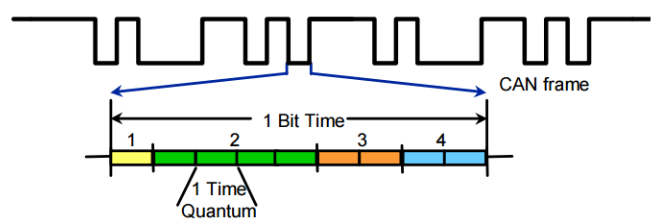
\includegraphics[width=0.75\textwidth]{img/time_quanta}
\end{center}
It is normally divided into four kind of field: \textit{synchronization segment}, \textit{propagation segment}, \textit{phase buffer segment 1} and \textit{phase buffer segment 2}. A \textit{bit} it is compose from 8 to 25 \textbf{time quanta} and it is the smallest discrete timing resolution used by CANBus node. Each \textbf{TQ} is generated by programmable divide of the oscillator. Each segment is composed by an integer number of TQs and segments are non-overlapping. The bitrate is selected by programming the width of the TQ and the number of TQ in the various segments.
\begin{enumerate}[nosep]
    \item \textbf{\textit{synchronization segment}}: it is used to synchronization the various node, only the receiver nodes have to adjust their own clock during the receiver of the payload. The lenght of the segment is always \textbf{1}.
    \item \textbf{\textit{propagation segment}}: if one node transmits to another faraway ones (geographically speaking) how we can synchronize the first \textit{TQ} of the \textit{synchronization segment}? The \textbf{propagation segment} allow the signal propagation across the network and through the nodes. This segment it could be compose from \textit{1 TQ} to \textit{8 TQs} and it is necessary to compensate for signal propagation delays on the bus line and through the electornic interface circuit of the bus nodes.
    \item \textbf{\textit{buffer segment one \& buffer segment two}}: this two segment it could have a programmable lenght between \textit{1 TQ} and \textit{8 TQs}. Between this two segment there is the \textbf{\textit{sample point}}. This point is used from the node to sample the information through the bus channel. This two segment are used to the \textbf{\textit{re-synchronization}}, in some circumstances we need to compensate the oscillator tolerances within the different CAN nodes. 
\end{enumerate}
\begin{boxA}
    \textcolor{red}{\textbf{Jump Width}} \\
    The \textit{jump width} is the amount of \textit{TQs} that we can add (in the \textit{phase buffer segment one}) or remove (in the \textit{phase buffer segment two}) that permit to adjust the lenght during the \textit{re-synch}.
\end{boxA}
Nowadays in many CANBus Modules the \textit{propagation time segment} and \textit{phase buffer segment one} are combined in a new segment named \textbf{\textit{timing segment 1}} (the \textit{phase buffer segment two} is renamed in \textbf{\textit{timing segment 2}}). \\ \newline
\textbf{\textit{Dynamic Sample Position}}: programming the sample point position allow \textbf{flexibility}:
\begin{enumerate}[nosep]
    \item \textbf{\textit{early sample}}: decrease the sensitivity to oscillator tolerances and permit to use lower cost oscillators.
    \item \textbf{\textit{late sampling}}: allow maximum signal propagation time (\textbf{reachability}), maximum bus lenght and poor bus topologies can be handled (more \textit{time quanta} in the \textit{propagation segment}).
\end{enumerate}
\textbf{\textit{CANBus Error}}: there are six possible different error:
\begin{enumerate}[nosep]
    \item \textbf{\textit{Bit-Error}}: write \textit{logical 0} over the bus and sense a \textit{logical 1} (or viceversa). In general if a transmitting ECU detects an \textbf{opposite bit} level on the CANBus we have a \textbf{bit-error}.
    \begin{itemize}[nosep]
        \item ECU writes \textit{logical 0} and reads \textit{logical 1} $\rightarrow$ very bad error.
        \item ECU writes \textit{logical 1} and reads \textit{logical 0} $\rightarrow$ it is ``possible'' when there is the \textbf{bitwise arbitration} or it is expected that the bus state will change to dominant as other nodes acknoledge the message
    \end{itemize}
    \item \textbf{\textit{Stuff Error}}: reminder on the \textit{bit stuffing}: it needs one opposite bit stuffed each 5 consecutive bits, it is used only from the beginning of the frame to the CRC delimiter. From the ACK field to the end is used the \textbf{fixed-form bit fields}. Each node receiving a message that breaks the bit stuffing rules will transmit an \textbf{error frame}.
    \item \textbf{\textit{Format Error}}: if one of the \textit{CRC delimiter field}, \textit{ACK field} or \textit{End Of Frame} have an divergent form, the receiving nodes perform a check to ensure these are correct, if not send a \textbf{error frame}.
    \item \textbf{\textit{CRC Error}}: \textit{CRC delimiter field} is the only weapon to ensure the integrity of the message, it depends on the polynomials division, if the \textit{CRC checks} (the reminder of message plus CRC divided by the Generator) is not $0$ it generates a \textbf{CRC Error}.
    \item \textbf{\textit{General Error}}: the seven \textbf{recessive} bits in the \textit{EOF} are used to inform the CANBus nodes about a general error occured during the transmission. If a receiver node found out an error, it writes six consecutive ``\textbf{zeros}'' forcing an error in the current frame that can be captured from everyone.
    \begin{figure}[h]
        \centering
        \begin{minipage}[t]{0.45\textwidth}
            \centering
            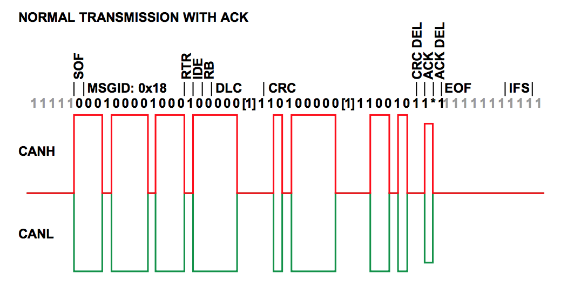
\includegraphics[width=\textwidth]{img/ok_ack}
        \end{minipage}
        \begin{minipage}[t]{0.45\textwidth}
            \centering
            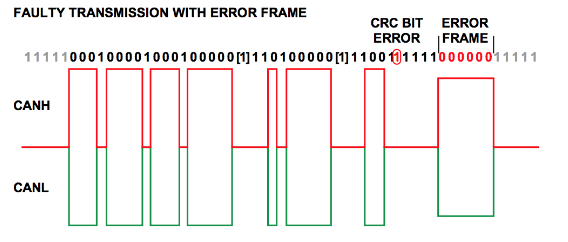
\includegraphics[width=\textwidth]{img/nok_ack}
        \end{minipage}
    \end{figure}
        
    \item \textbf{\textit{ACK Error}}: it happen when no one of the receiver nodes write on the buses an \textbf{dominant} bit in the \textit{ACK field} of the transmitting frame. \\
    \begin{boxA}
        \textbf{\textit{CANBus ACK}} \\
        The transmitting nodes, after the DATA and the CRC, write in the bus a \textit{logical 1} (\textbf{recessive}) and it hopes, in the mean time, that \textbf{at least} one receiver write a \textit{logical 1} (\textbf{dominant}) in the ACK bit, if not the transmitting node (reads on the bus \textit{logical 1}) and will resend the message. \\
        There is two bits for the \textit{ACK field} to absorbe possible delay. We need to allocate space for ``not perfect synchronized receiver'' to push a \textbf{dominant} bit on the bus.
    \end{boxA}
    The \textit{ACK} is triggered by another node so the voltage value could be slightly different. These technologies have some implication on the CANBus protocol, like:
    \begin{itemize}[nosep]
        \item also the recevier node/s can (have to) transmit during specific frame slot (the \textit{ACK field} or \textit{EOF}).
        \item all the receiver must check the \textit{CRC} very quickly in order to know if the message have pass the integrity checks.
        \item a CANBus network \textbf{\textit{must have at least two nodes to work}}, because with only one node no one can acknoledge a message.
    \end{itemize}
\end{enumerate}
For the calculous of the time in the circuit (in the CANBus controller) it is normally used \textbf{\textit{time crystal}}, the smallest \textit{ICs} possible is the $8MHz$ \textit{time crystal}. If we consider each clock cycle for the smallest unit in CANBus (\textit{time quanta}) for each bit we have at least \textit{8 TQs} (up to \textit{25 TQs}). \\
If we minimize the size of the of a single bit we have to consider \textit{8 TQs}. $\frac{8MHz}{8 TQs} = 1MHz$ we can obtain the maximum bitrate for the CANBus. \\ \newline
\textbf{CANBus Recap}:
\begin{enumerate}[nosep]
    \item \textbf{\textit{low cost}}: the price is \textbf{always} a costraint, with it's two wires has a good price-performance tradeoff. This enables the use of CANBus outside the autonomotive domain.
    \item \textbf{\textit{reliability}}: CANBus has sophisticated error detection and handling mechanisms. If failed the integrity checks of the frame it could repeat the sending of the same data and every nodes are informed about the error. CANBus has high immunity to EMI.
    \item \textbf{\textit{latency}}: CANBus means real-time (soft) because there is low latency between transmission and request and actual start of transmission. CANBus has inherent arbitration on message priority due to the bitwise arbitration logic.
    \item \textbf{\textit{flexibility \& speed}}: CANBus nodes are ``plug \& play'' and there are not limited number of nodes into a network.
    \item \textbf{\textit{multi master operation}}: (ECU peers) each nodes is able to access to the bus, if there is a fulty nodes the bus communication is not disturbed and they switch-off from the communication.
    \item \textbf{\textit{broadcast capabilities}}: message can be sento to single/multiple nodes and every node simultaneously receive common data. 
    \item \textbf{\textit{Standardize}}: \textit{ISO-DIS 11898} (high speed), \textit{ISO-DIS 115192-2} low speed.
\end{enumerate}

\newpage
\section{Controller Area Network Flexible Data-Rate}
The \textbf{\textit{CAN-FD}} is the evolution of the \textit{CANBus}. The mainly disadvantages of CANBus are: $1MHz$ in some circumstances are not enough and only \textit{8 bytes} of payload are often restrictive. To be compliant to standard CANBus the \textit{arbitration phase} (before the data) and \textit{ACK phase} (after the data) must be mantein to the same frequency. \\
CAN-FD data frames can be transmitted with two different bit-rates, in the \textit{arbitration phase} and in the \textit{ACK phase} the bitrate depends on the network topology and it is limited to $1MHz$, instead in the \textit{data phase} the bitrate is limited by the \textit{transceiver characteristics}:
\begin{itemize}[nosep]
    \item support a bitrate higher than $1MHz$.
    \item support a payload larger than \textit{8 bytes}.
\end{itemize}
The increase of the frame speed is possible by shortening the bit time. We define the \textbf{\textit{Bit Rate Shift - BRS}} is the bit in the \textit{control field} used to inform \textbf{ALL} the nodes that sender will transmit faster in the \textit{data transmission phase} and the \textbf{\textit{Extended Data Lenght - EDL}}. The implication of this change are:
\begin{itemize}[nosep]
    \item \textbf{larger payload}: it needs more \textit{CRC bits} to maintain the robustness of CANBus, to have more \textit{CRC bits} it needs a \textbf{larger generator}.
    \item \textbf{shorter bit-time}: new bit-time logic in the state machine, a \textit{factor} is introduce between the bit time during arbitration phase and the bit-time during the transmission. The tipical factor is 8 $\rightarrow$ considerering the fastest rate of CANBus \textit{arbitration phase} and the longer header and CRC, the final result is more or less $6MHz$.
\end{itemize}
\begin{figure}[h]
    \centering
    \label{img:canfd}
    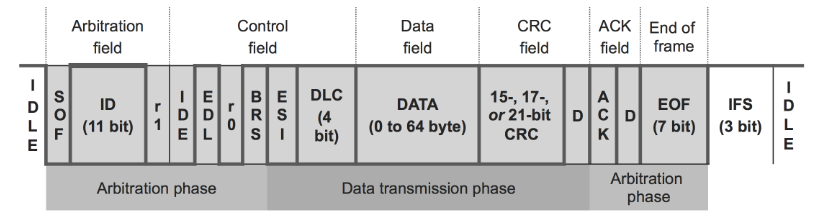
\includegraphics[width=0.75\textwidth]{img/can_fd}
\end{figure}
To summarize the \textbf{CAN-FD} could reach in the \textit{data transmission phase} the speed transmission of $6MHz$ and the possibility of sending a payload large up to \textbf{64 bytes}

\newpage
\section{Local Interface Network}
\begin{center}
    \label{fig:can_lin}
    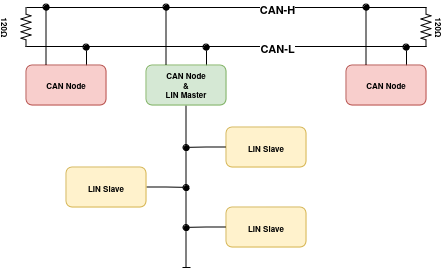
\includegraphics[width=0.5\textwidth]{img/can_lin}
\end{center}
The \textbf{\textit{LIN}} is a message oriented communication protocol that is design and developed to create something cheaper than low speed CANBus, this purpose it was reach partaway. Like the CANBus, LIN, works on the first two layers of the ISO/OSI stack (physical and data link layers), but it uses a \textbf{master-slave} concept. Using this architecture, the LIN busses, can have only a quartz on the master that manage the synchronization on all the LIN network, to achieve without waste space on the vehicle, the master of the LIN mesh is part of the CANBus network. This is the reason why the LIN is also know like a \textbf{\textit{sub bus}} of CANBus (Fig. \ref{fig:can_lin}). As result on the communication we can say that LIN network is self-synchronize, but for this reason it needs to have lax timing constraints because only one node (the \textbf{master}) can schedule the order of the transmission. In addition to this, LIN busses, has other difference between CANBus:
\begin{itemize}[nosep]
    \item LIN is a \textbf{bidirectional one-wire line} and it can reach the frequency up to $20kHz$ (CANBus can reach $1MHz$).
    \item The \textbf{voltage} for the analog transmission over the channel is 40V, instead the CANBus is only up to 5V.
    \item \textbf{Bit Transmission} is \textit{UART} like:
    \begin{center}
        \begin{tabular}{ | c | c | c | } \hline
            \multicolumn{3}{|c|}{\textbf{bit transmission}} \\ \hline
            1 bit & 8 bits & 1 bit \\ \hline
            \textbf{start bit} & \textbf{data bits} & \textbf{stop bit} \\ \hline
        \end{tabular}
    \end{center}
\end{itemize}
In LIN protocol there is a rudimental error detection on the frame, it is a sum of all the payload bytes modulo 256 (in this way it can be stored into a single byte), but also on the channel, if a sender while monitoring the bus, read an unexpected state abort the communication without correction. The \textbf{schedule} of the network is hardcoded on the \textbf{master's firmware} (static), the scheduler determines which node have to transmit in that specific slice of time. This consent to have a channel that is \textbf{mostly deterministic}, permit to the slave to not know how it is schedule the transmission and allow to the master to \textit{change the order of transmission runtime}. \\ \newline
\textbf{\textit{LIN Message}}: is divide into two component: \textit{Message Header} and \textit{Message Response}. The first one is sent over the channel by the \textbf{maaster node} and is like a request for a specific slave, instead it is possible to see the second one like the slave response.
\begin{center}
    \begin{tabular}{ | p{2cm} | p{1cm} | p{2cm} | p{5cm} | p{2cm} | } \hline
        \multicolumn{3}{|c|}{\textbf{Message Header}} & \multicolumn{2}{|c|}{\textbf{Message Response}} \\ \hline
        \textit{Break} & \textit{Sync} & \textit{Identifier} & \textit{Data} & \textit{Checksum} \\ \hline
        14 bits & 8 bits & 8 bits & 0 to 64 bits & 8 bits \\ \hline
    \end{tabular}
\end{center}
Description for each field:
\begin{enumerate}[nosep]
    \item \textbf{\textit{Break}}: is composed by two kinds of fields: \textbf{13 low bits} (\textit{dominant}) and \textbf{1 high bit} (\textit{recessive}) that is used to delimiter of the field.
    \item \textbf{\textit{Sync}}: is used to \textit{synchronize} the bit timing of the slave, it is always \textbf{0x55} (01010101) in this way follow the profile of the clock.
    \item \textbf{\textit{ID}}: is used to individuate the right slave, different from the CANBus, in this identifier there are parity bit, to have a check on the integrity of the ID, because in this case is very important for the correct master-slave communication (\textbf{protected field}). ID is divide in two segment:
    \begin{itemize}[nosep]
        \item from \textbf{LIN 2.0} the first \textbf{2 MSB bits} define the lenght of the payload that could be 2, 4 or 8 bytes, previous version of LIN used static 8 bytes data lenght.
        \item \textbf{4[6] bits} for the ``real'' ID.
        \item \textbf{2 parity bits}:
        \begin{center}
            $p_0 = id_0 \oplus id_1 \oplus id_2 \oplus id_4$ \\
            $p_1 = id_1 \oplus id_3 \oplus id_4 \oplus id_5$
        \end{center}
    \end{itemize}
    \item \textbf{\textit{Data}}: contain the payload, and it was send by the slave selected by the master with the lenght settled in the identifier.
    \item \textbf{\textit{Checksum}}: is this case, like said before, the checksum is the sum of all the payload bytes modulo 256, in that way it can be stored into a single byte.
    \begin{center}
        \begin{tabular}{ | c |  c |  c |  c |  c |  c |  c |  c |  c | } \hline
            & $d_7$ & $d_6$ & $d_5$ & $d_4$ & $d_3$ & $d_2$ & $d_1$ & $d_0$ \\ \hline
            \textbf{carry} & & \textcolor{red}{\textit{1}} & \textcolor{red}{\textit{1}} & \textcolor{red}{\textit{1}} & & \textcolor{red}{\textit{1}} & & \\ \hline
            \textbf{first byte} & 0 & 0 & 0 & 1 & 0 & 1 & 1 & 0 \\ \hline
            \textbf{second byte} & 0 & 0 & 0 & 1 & 0 & 1 & 1 & 1 \\ \hline
            \textbf{third byte} & 0 & 0 & 0 & 1 & 0 & 1 & 1 & 0 \\ \hline
            \textbf{forth byte} & 0 & 0 & 0 & 1 & 0 & 0 & 0 & 0 \\ \hline
            \textbf{fifth byte} & 0 & 0 & 0 & 1 & 0 & 0 & 0 & 0 \\ \hline
            \textbf{\textit{checksum}} & \textbf{0} & \textbf{1} & \textbf{1} & \textbf{0} & \textbf{0} & \textbf{0} & \textbf{1} & \textbf{1} \\ \hline
        \end{tabular}
    \end{center}
\end{enumerate}
LIN nodes are typically bundled in clusters each with a master that interfaces with the backbone CANBus. We have introduce the general message/frame format, but in LIN protocol there are six kinds of different messages (encoded in the ID field):
\begin{enumerate}[nosep]
    \item \textbf{\textit{Unconditional Frames}}: is defined by the ID \textbf{\textit{0x00 - 0x3B}} and is the default type of frame, where the master send a header over the channel and the request slave reply.
    \item \textbf{\textit{Event Trigger Frames}}: is defined by the ID \textbf{\textit{0x00 - 0x3B}}, the master polls multiple slaves, the slave who have updated data response, if there are collision, the communication end and the master switch to \textit{unconditional frame}.
    \item \textbf{\textit{Sporadic Frames}} is defined by the ID \textbf{\textit{0x00 - 0x3B}} in this type of message the master acts like a slave and reply to his own requests.
    \item \textbf{\textit{Diagnostic Frames}} is defined by the ID \textbf{\textit{0x3C - 0x3D}} with this frame the communication becomes request-response, the \textbf{\textit{0x3C}} is the ID where the master make the request, instead the \textbf{\textit{0x3D}} is the ID where the slave reply.
    \item \textbf{\textit{User Defined Frames}} is define by the ID \textbf{\textit{0x3E}} is a user-defined frame and it can contain any types of information.
    \item \textbf{\textit{Reserved Frames}}: ID \textbf{\textit{0x3F}}
\end{enumerate}
There is a reason why the \textbf{data lenght} of CANBus and LIN are equal. Since LIN is also called CANBus sub system, for compatibility reason the payload is equal. Message of CANBus can be sent over LIN too and viceversa.


% PAGINA VUOTA
%\clearpage\null\thispagestyle{empty}\clearpage
%\appendix
%\appendixpage
%\addappheadtotoc

%\clearpage\null\thispagestyle{empty}\clearpage


%\listoffigures


\begin{flushleft}
\bibliographystyle{plain}
\bibliography{sections/references} 
\end{flushleft}

\end{document}
